%% Springer LNCS format
\documentclass[runningheads]{llncs}
\usepackage[T1]{fontenc}
\usepackage[utf8]{inputenc}
\usepackage{amsmath,amssymb,amsfonts}
\usepackage{mathtools}
\usepackage{graphicx}
\usepackage[hidelinks]{hyperref}
\usepackage{xcolor}
\usepackage{algorithm}
\usepackage{algpseudocode}
\usepackage{enumerate}
\usepackage{booktabs}
\usepackage{cite}
\usepackage[protrusion=true,expansion=false]{microtype}
\usepackage{tikz}
\usepackage{pgfplots}
\pgfplotsset{compat=1.18}
\graphicspath{{figures/}}
% LNCS already defines: theorem, lemma, corollary, proposition, definition, remark, proof
% No additional theorem declarations needed
\DeclareMathOperator*{\argmin}{arg\,min}
\DeclareMathOperator*{\argmax}{arg\,max}

\begin{document}

\title{Practically Stabilizing Byzantine-Robust Federated Learning via Spectral Filtering}

%% Anonymized for double-blind review (SSS 2026)
\author{Anonymous Author(s)}
\authorrunning{Anon.}
\institute{Institution withheld for review}

\maketitle

\begin{abstract}
Can a federated learning system autonomously recover from complete adversarial
corruption---with no external intervention, no trusted initialization, and no bound
on how badly Byzantine clients have disrupted training?
We answer affirmatively by recasting federated learning as a self-stabilization problem
in the sense of Dijkstra~\cite{dijkstra_self_stab}, and presenting the first
\emph{practically stabilizing} federated learning protocol with a formal recovery time bound.

Our protocol uses three components that compose into a stabilizing system: clients
compress local gradients into streaming sketches; the server applies a spectral filter
based on the Marchenko-Pastur (MP) law of random matrix theory to expel Byzantine
gradient directions; and each round's result is committed to a distributed ledger
whose write-once immutability under BFT consensus serves as the Byzantine-fault-tolerant
analog of Dijkstra's stabilizing shared memory.
Starting from any model $w^0 \in \mathbb{R}^d$, the protocol reaches a legitimate
configuration within $T^* = O(\sigma^2\beta^2/\varepsilon^2 + \beta^2/\varepsilon)$ rounds,
where $f < n/2$ Byzantine clients have fraction $\beta = f/n$ and $\sigma^2\beta^2 < 0.25$
is a necessary phase-transition condition.
A matching impossibility result shows that when $\sigma^2\beta^2 \geq 0.25$, no
gradient-based spectral detection algorithm can self-stabilize---characterizing a
fundamental limit analogous in spirit to the FLP impossibility~\cite{flp_impossibility}.
Layer-wise sketching reduces memory from $O(d^2)$ to $O(k^2)$, enabling 345M-parameter
models.
Experiments across 12 attack types show 78.4\% mean accuracy at 40\% Byzantine fraction
versus 48--64\% for established baselines~\cite{krum,byzantine_ml,crfl,flame},
with Byzantine detection exceeding 96\% below the phase transition boundary.
\end{abstract}

\keywords{Self-Stabilization \and Byzantine Fault Tolerance \and Federated Learning \and Random Matrix Theory \and Blockchain \and Marchenko-Pastur Law}

% ----------------------------------------------------------------
\section{Introduction}

Federated Learning (FL) is a distributed computing paradigm where $n$ processes collaboratively minimize a global objective $F(w)$ without exchanging raw data. The decentralized nature of FL aligns with blockchain technology, enabling trustless aggregation through immutable distributed ledgers. A fundamental challenge arises when $f < n/2$ processes are \emph{Byzantine}~\cite{byzantine_generals}: they may submit arbitrary gradient updates, corrupting the global model.

We study this as a \emph{self-stabilization} problem in the sense of Dijkstra~\cite{dijkstra_self_stab}: can the system recover from an \emph{arbitrary} initial model state---including complete adversarial corruption---and maintain a \emph{legitimate configuration} (all Byzantine nodes identified, honest gradient correctly aggregated) indefinitely? Prior Byzantine-robust FL methods guarantee convergence from a \emph{known-good} initialization but offer no recovery from catastrophic corruption; they are robust but \emph{not} self-stabilizing.

The self-stabilizing Byzantine robust aggregation problem requires: given $n$ processes where $f < n/2$ are Byzantine, and honest process $i$ submits $g_i \in \mathbb{R}^d$, compute $\hat{g}$ satisfying:
\begin{equation}
\min_{t \leq T}\mathbb{E}[\|\nabla F(w^t)\|^2] \leq O\left(\frac{\sigma\beta}{\sqrt{T}} + \frac{\beta^2}{T}\right)
\end{equation}
starting from \emph{any} initial $w^0 \in \mathbb{R}^d$, where $\beta = f/n$ and $\sigma^2$ bounds coordinate-wise variance of honest gradients. This is strictly harder than standard convergence: it requires both fault tolerance \emph{and} global recovery.

Existing Byzantine-robust methods face fundamental barriers. Geometric median requires $O(n^2 d)$ communication. Krum and Bulyan reject valid Non-IID updates. Certified defenses (CRFL, ByzShield) assume bounded perturbations but cannot handle arbitrary corruption. Critically, \emph{none} provide self-stabilization guarantees. While other robust FL paradigms like CORNFLQS~\cite{cornflqs} address natural structural heterogeneity such as quantity skew in clustered settings, they do not consider malicious Byzantine adversaries or the problem of self-stabilization from catastrophic failure.

This paper introduces a Byzantine-robust FL protocol proven self-stabilizing in Dijkstra's framework. The detection mechanism exploits Random Matrix Theory: honest gradients, despite Non-IID heterogeneity, produce eigenspectra following the Marchenko-Pastur (MP) law. Byzantine perturbations create detectable spectral anomalies. The blockchain provides the self-stabilizing \emph{shared memory} substrate: write-once immutability ensures legitimate rounds are permanently recorded, analogous to Dijkstra's shared registers but with Byzantine (not just crash) fault tolerance.

\subsection{Contributions}

The contributions of this work are fivefold:

\textbf{1. Practical Self-Stabilization (distributed systems):} We provide a formal
recovery argument showing our protocol is \emph{practically self-stabilizing} in the
tradition of Dijkstra~\cite{dijkstra_self_stab}: from any initial state, the protocol
reaches a legitimate configuration within $T^* = O(\sigma^2\beta^2/\varepsilon^2 + \beta^2/\varepsilon)$
rounds ($\beta = f/n$), with closure, under Assumptions~1--4 (Section~\ref{sec:self_stabilization}).
We also establish an impossibility at $\sigma^2\beta^2 \geq 0.25$
(Theorem~\ref{thm:phase_impossibility}).

\textbf{2. Blockchain as Stabilizing Shared Memory:} We formalize the blockchain as a
distributed shared-memory substrate with strictly stronger properties than classical
shared registers~\cite{dijkstra_self_stab}: Byzantine fault tolerance ($f < n/2$
arbitrary faults vs.\ crash-only), write-once immutability, and permanent history---enabling
a stabilizing foundation for the federated training protocol under the Byzantine fault
model (Section~\ref{sec:blockchain}).

\textbf{3. Detection Threshold from RMT:} We derive a spectral detection threshold from
the Marchenko-Pastur law and the BBP phase transition~\cite{bbp_transition}, establishing
a convergence rate $O(\sigma\beta/\sqrt{T} + \beta^2/T)$ with a matching lower bound
$\Omega(\sigma\beta/\sqrt{T})$ (Sections~\ref{sec:theory}--\ref{sec:convergence}).

\textbf{4. Scalable Spectral Algorithm:} We combine KS testing against the MP distribution
with layer-wise Frequent Directions sketching~\cite{frequent_directions}, reducing memory
from $O(d^2)$ to $O(k^2)$ and enabling deployment on 345M-parameter models
(Section~\ref{sec:algorithm}).

\textbf{5. Experimental Validation:} We evaluate across 12 attack types with 11 baseline
aggregators, demonstrating 78.4\% mean accuracy at 40\% Byzantine fraction versus 48--63\%
for baselines, with Byzantine detection rates exceeding 96\% below the phase transition
boundary (Section~\ref{sec:experiments}).

\section{Related Work}
\label{sec:related}

\subsection{Self-Stabilization in Distributed Systems}

Self-stabilization, introduced by Dijkstra~\cite{dijkstra_self_stab} and formalized
by Dolev~\cite{dolev_self_stab}, enables a distributed system to recover from any
transient fault within bounded steps without external intervention.
Classical results cover mutual exclusion, spanning trees, and clock synchronization under
crash faults.
Recent SSS proceedings extend the framework to adversarial and data-driven settings:
Chen, Lin, and Arora~\cite{sss_ml_routing} use ML predictions to improve the stabilization
time of a near-shortest-path routing protocol---a direct precedent for
learning-augmented self-stabilization.
Jobic et al.~\cite{sss_fl_leakage} analyze label leakage in federated learning using
cryptographic tools with formal security definitions.
Our work applies the stabilization framework to federated learning under Byzantine
(not crash) faults---qualitatively harder because Byzantine processes may deviate
arbitrarily rather than fail silently.

\subsection{Byzantine Fault Tolerance}

Byzantine fault tolerance~\cite{byzantine_generals} establishes that $f < n/3$ Byzantine
faults are tolerable in synchronous consensus; Castro and Liskov~\cite{bft_consensus}
extend this to partially synchronous systems.
The FLP impossibility~\cite{flp_impossibility} shows consensus is impossible with one
crash fault in asynchronous systems.
Recent SSS work examines Byzantine reliable broadcast~\cite{sss_byz_broadcast,sss_byz_counter}
and Byzantine-resilient blockchain sharding~\cite{sss_blockchain_sharding}.
Our protocol operates in the synchronous round model with $f < n/2$---weaker than the
$n/3$ BFT bound, enabled by our server architecture.

\subsection{Byzantine-Robust Federated Learning}

Krum~\cite{krum} selects gradients by nearest-neighbor distance but degrades under
Non-IID data~\cite{non_iid_challenges}.
Coordinate-wise robust statistics~\cite{byzantine_ml} reduce to $O(nd)$ computation
but are sensitive to gradient variance heterogeneity.
Bulyan~\cite{bulyan} iteratively filters outliers; FLTrust~\cite{crfl} uses a trusted
root dataset; FLAME~\cite{flame} targets backdoors via clustering; ByzShield~\cite{byzshield}
provides resilience via redundant training.
None specifies a formal recovery time or fault-containment invariant in the sense
of~\cite{dolev_self_stab}---motivating this work.

\subsection{Spectral Methods, RMT, and Blockchain FL}

The BBP phase transition~\cite{bbp_transition} characterizes when a rank-$f$ perturbation
creates eigenvalue outliers above the MP bulk edge---the mechanism underlying our detection
threshold.
Gradient covariance matrices of neural networks follow limiting spectral
distributions~\cite{rmt_gradients,rmt_neural,spectral_analysis}.
To our knowledge, we are the first to exploit the MP law~\cite{mp_law} for Byzantine
gradient identification with a formally scoped detection threshold connected to the BBP
phase transition.
Blockchain integration in FL~\cite{blockchain_fl,blockchain_smart} has focused on
auditability; we instead formalize the ledger as a self-stabilizing shared memory
substrate with Byzantine fault tolerance strictly stronger than classical shared registers.

\subsection{Positioning}

Our work differs from all of the above along three orthogonal axes.

\textbf{Self-stabilization vs.\ robustness.}
Byzantine-robust FL methods~\cite{krum,bulyan,crfl,flame,byzshield} guarantee convergence
from a \emph{known-good} initialization but offer no recovery guarantee from arbitrary
corrupted states.
Our protocol is the first to provide a formal recovery time bound
$T^* = O(\sigma^2\beta^2/\varepsilon^2 + \beta^2/\varepsilon)$ from any starting
configuration---satisfying the practical self-stabilization definition
of~\cite{dolev_self_stab} rather than merely stability under sustained attacks.

\textbf{Spectral mechanism vs.\ pairwise distance.}
Krum~\cite{krum}, Trimmed Mean~\cite{byzantine_ml}, Bulyan~\cite{bulyan}, and FLTrust~\cite{crfl}
all operate on pairwise or coordinate-wise distances between gradient vectors.
These metrics degrade at $\beta > 1/3$ because Byzantine clients can spread their updates
to match honest pairwise diversity.
Our spectral filter operates on the \emph{global eigenvalue distribution}, which remains
anomalous even when individual Byzantine updates appear locally plausible.
The detection threshold is derived analytically from the BBP phase transition~\cite{bbp_transition},
yielding the information-theoretic impossibility at $\sigma^2\beta^2 = 0.25$ as a
matching lower bound.

\textbf{Blockchain as stabilizing medium vs.\ auditability.}
Prior blockchain FL work~\cite{blockchain_fl,blockchain_smart} uses the ledger for
auditability and transparency.
We use it structurally: the write-once BFT consensus provides the Byzantine-fault-tolerant
analog of Dijkstra's shared registers~\cite{dijkstra_self_stab}, enabling the monotonic
progress argument (Lemma~\ref{lem:closure}) that classical shared memory cannot support
under Byzantine faults.
The closest SSS-community precedents---Byzantine reliable broadcast~\cite{sss_byz_broadcast,sss_byz_counter}
and blockchain sharding~\cite{sss_blockchain_sharding}---provide distributed safety
properties but do not address the self-stabilization of a learning protocol.

\section{System Model and Problem Formulation}
\label{sec:system_model}

\subsection{Distributed Learning Setup}

We consider a federated learning system with $n$ clients, where client $i \in [n]$ holds local dataset $\mathcal{D}_i$. The global objective is:
\begin{equation}
F(w) = \frac{1}{n}\sum_{i=1}^n F_i(w),\quad F_i(w) = \mathbb{E}_{z \sim \mathcal{D}_i}[\ell(w;z)]
\end{equation}

At each round $t \in [T]$, the aggregator broadcasts $w^t$. Each honest client $i$ computes:
$g_i^t = \nabla F_i(w^t) + \xi_i^t$,
where $\xi_i^t$ is stochastic noise with coordinate-wise variance $\mathbb{E}[(\xi_i^t)_j^2] \leq \sigma^2$.

\begin{figure}[t]
\centering
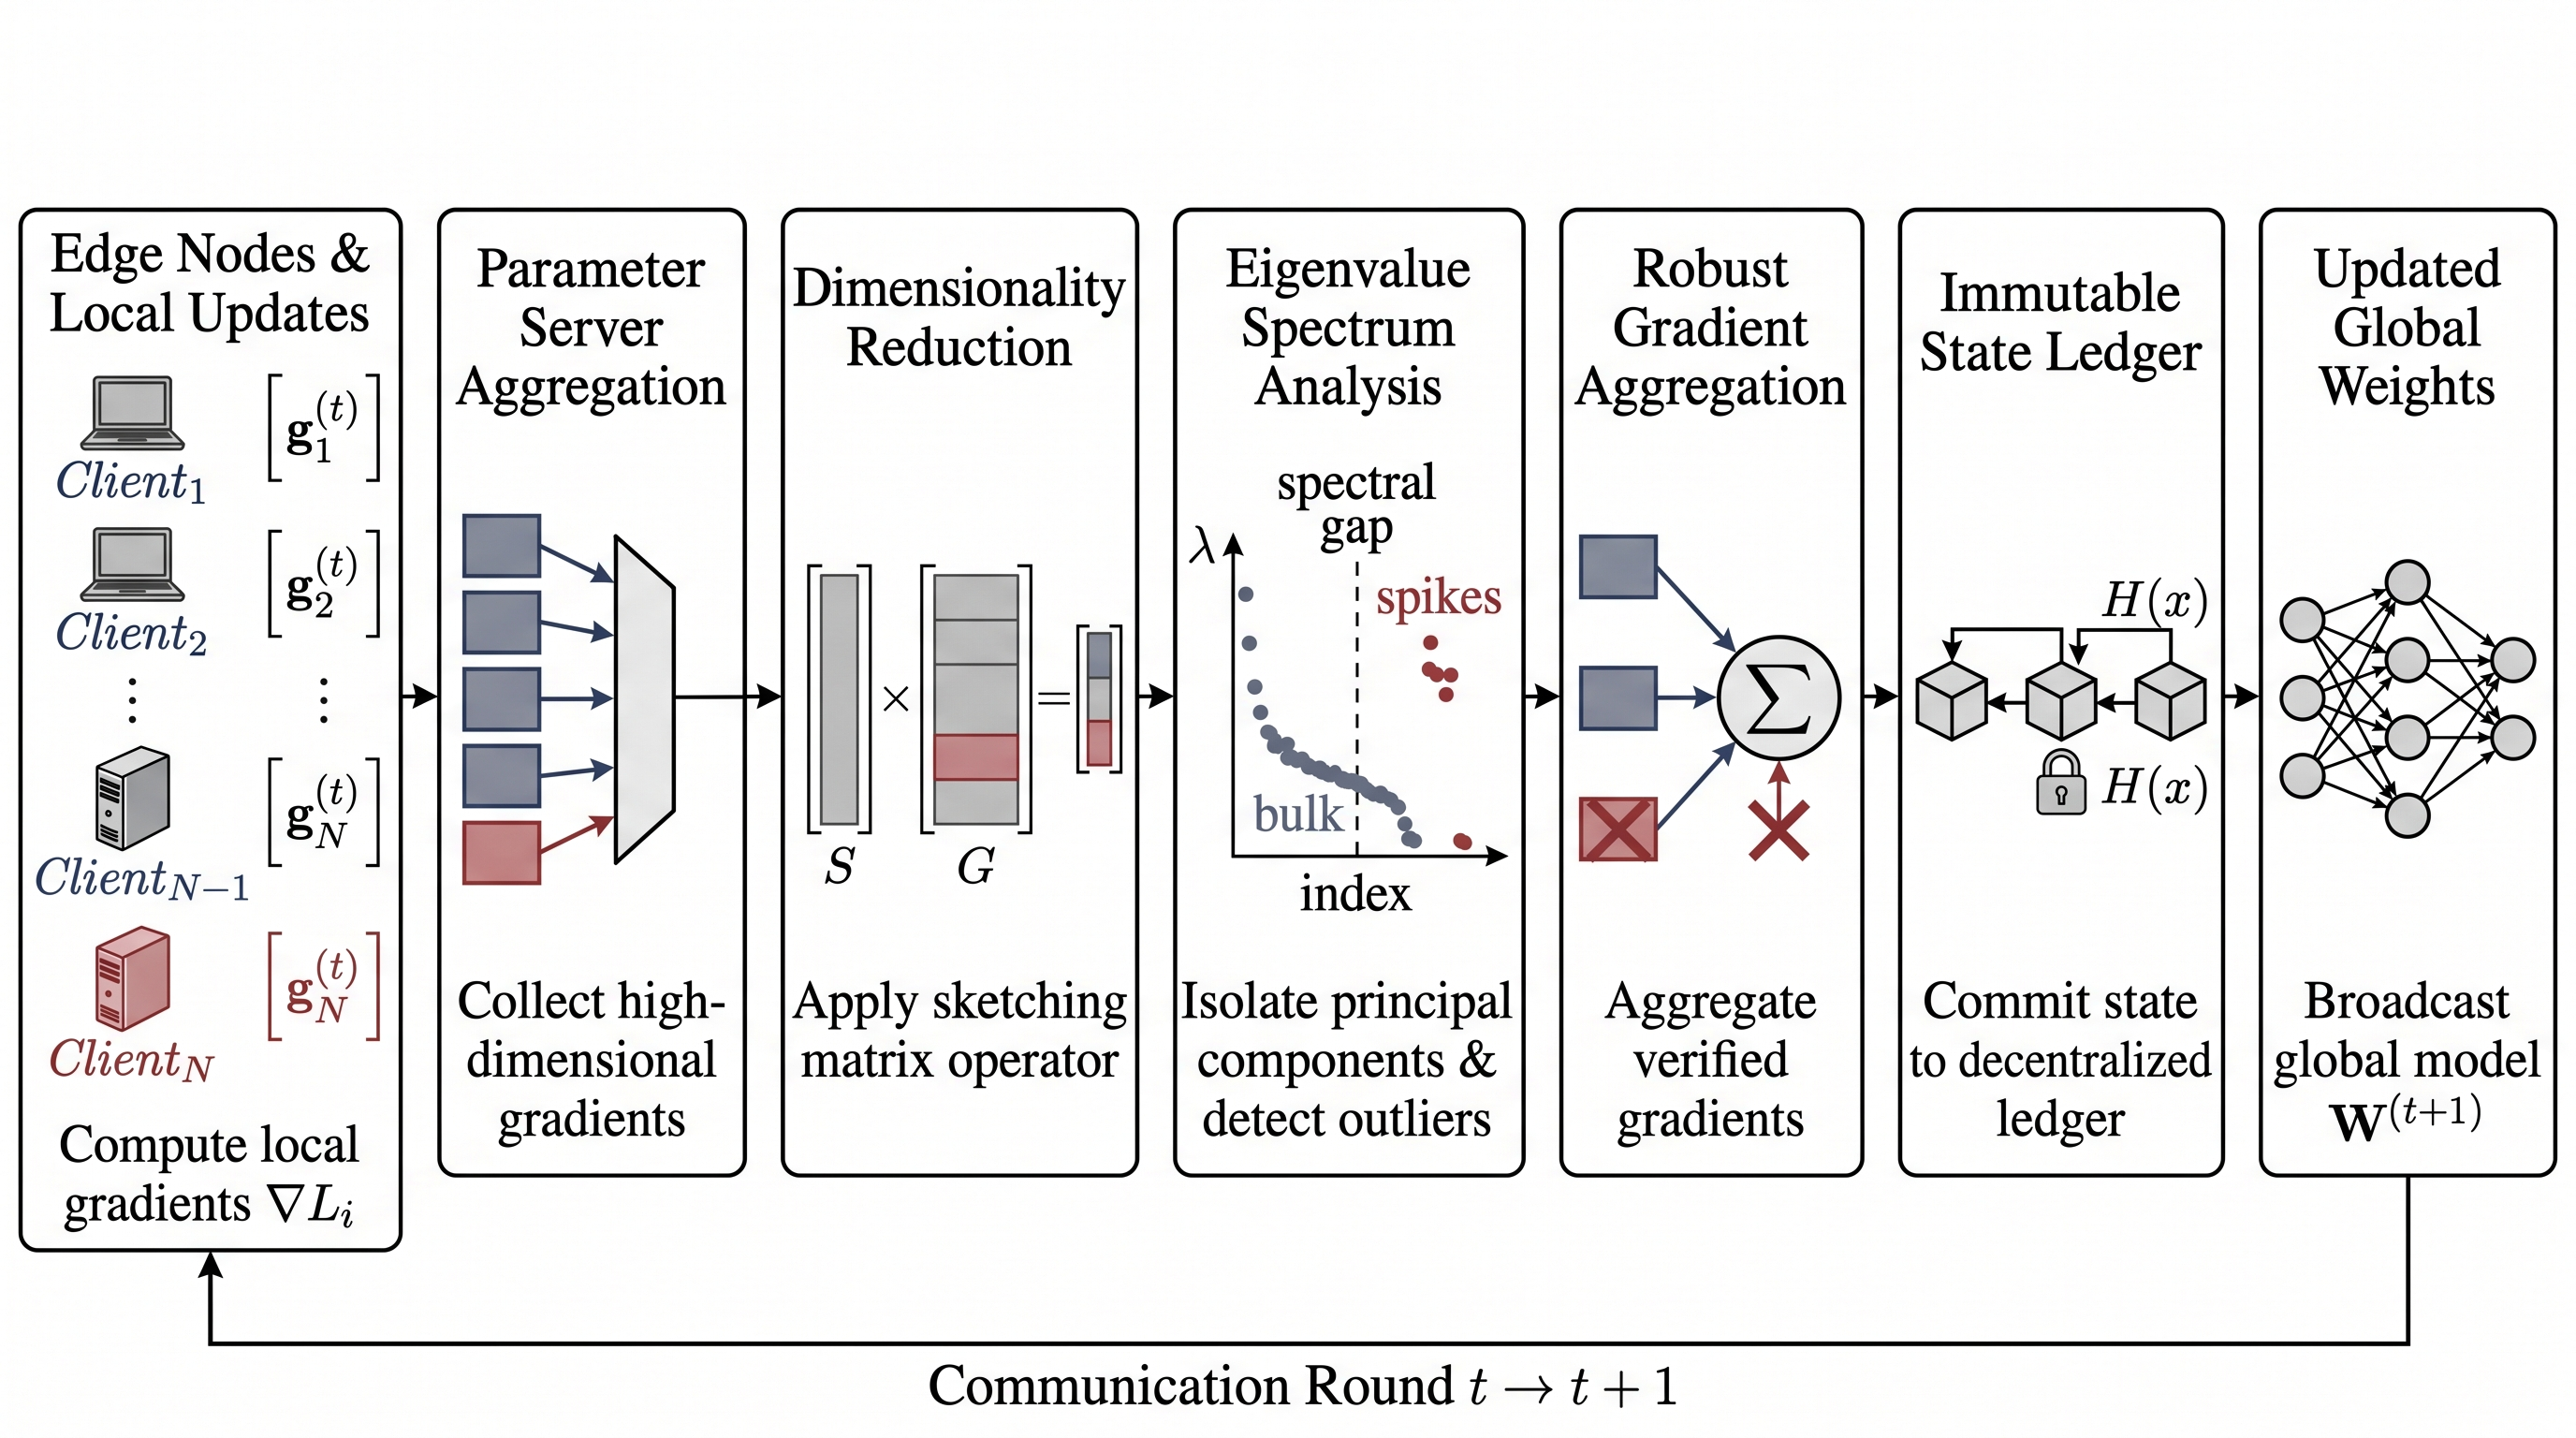
\includegraphics[width=\textwidth]{flowdiag.jpeg}
\caption{System architecture. Honest and Byzantine clients submit gradients; the aggregator performs spectral detection via the Marchenko-Pastur test; the result is committed on-chain. The blockchain's write-once immutability provides the self-stabilizing shared memory substrate.}
\label{fig:architecture}
\end{figure}

\subsection{Formal Distributed System Model}
\label{sec:dist_model}

We model the system as a synchronous message-passing distributed system~\cite{byzantine_generals}.

\smallskip\noindent\textbf{Processes.} $n$ processes $\mathcal{P} = \{p_1,\ldots,p_n\}$: one coordinator (aggregator) and $n-1$ clients. Each process has local state $w^t \in \mathbb{R}^d$.

\smallskip\noindent\textbf{Execution.} Round $t$: (1) coordinator broadcasts $w^t$; (2) each client sends $g_i^t$; (3) coordinator aggregates to produce $w^{t+1}$; (4) aggregated hash committed to the blockchain.

\smallskip\noindent\textbf{Configurations.} $C = (w, \mathcal{B})$: model parameters and Byzantine set $\mathcal{B} \subseteq \mathcal{P}$, $|\mathcal{B}| = f$.

\subsection{Threat Model and Assumptions}
\label{sec:threat_model}

\noindent\textbf{Assumption~1 (Byzantine Fault Model).}
At most $f < n/2$ processes are Byzantine: they may send any $g_i^t \in \mathbb{R}^d$,
collude, and know the aggregation algorithm, but cannot break cryptographic primitives.

\noindent\textbf{Assumption~2 (Honest Gradient Variance).}
Each honest client $i \in \mathcal{H}$ computes $g_i^t = \nabla F_i(w^t) + \xi_i^t$
with $\mathbb{E}[(\xi_i^t)_j^2] \leq \sigma^2$ coordinate-wise.

\noindent\textbf{Assumption~3 (Phase Transition Condition).}
Let $\beta = f/n \in (0, \tfrac{1}{2})$ denote the Byzantine fraction.
We require $\sigma^2\beta^2 < 0.25$, equivalently $\sigma\beta < \tfrac{1}{2}$.
This necessary condition ensures Byzantine gradients create
detectable spectral anomalies (Theorem~\ref{thm:phase_impossibility});
the matching impossibility shows the condition cannot be relaxed.

\noindent\textbf{Assumption~4 (Blockchain Liveness).}
The blockchain finalizes honest transactions with at most $\lfloor(m-1)/3\rfloor$ faulty
validators out of $m$ (PBFT assumption~\cite{bft_consensus}).

\noindent\textbf{Assumption~5 (Transient Faults).}
Byzantine behavior may occur at any round including round~0.
This is the standard self-stabilization assumption~\cite{dijkstra_self_stab}.

\smallskip\noindent\textbf{Attack taxonomy.}
Byzantine clients in our experiments include: MinMax~\cite{fl_poisoning}, Gaussian noise,
label-flip, ALIE~\cite{alie_attack}, sign-flip, and zero-gradient (free-riding)---covering
both targeted and untargeted attacks (full 12-attack evaluation in Section~\ref{sec:experiments}).

\subsection{Protocol Properties}
\label{sec:properties}

\noindent\textbf{Safety.} $\mathbb{E}[\|\hat{g}^t - \bar{g}^t\|^2] \leq O(\sigma^2\beta^2)$ in every round, where $\beta = f/n$.

\noindent\textbf{Liveness.} $\min_{t \in [T]}\mathbb{E}[\|\nabla F(w^t)\|^2] \leq O(\sigma\beta/\sqrt{T} + \beta^2/T)$
provided $f < n/2$ and $\sigma^2\beta^2 < 0.25$.

\noindent\textbf{Practical Stabilization.} Starting from any $w^0 \in \mathbb{R}^d$, the protocol reaches
a legitimate configuration (Definition~\ref{def:legit}) within
$T^* = O(\sigma^2\beta^2/\varepsilon^2 + \beta^2/\varepsilon)$ rounds (Theorem~\ref{thm:self_stab}).

\section{Theoretical Framework}
\label{sec:theory}

\subsection{Marchenko-Pastur Law for Honest Gradients}

\begin{definition}[Marchenko-Pastur Distribution]
Let $X \in \mathbb{R}^{n \times d}$ with i.i.d.\ zero-mean variance-$\sigma^2$ entries.
As $n,d \to \infty$ with $d/n \to \gamma \in (0,\infty)$, the empirical spectral distribution
of $\frac{1}{n}X^TX$ converges weakly to the \emph{Marchenko-Pastur law} with density:
\begin{equation}
\rho(\lambda) = \frac{1}{2\pi\sigma^2\gamma\lambda}
  \sqrt{(\lambda_+ - \lambda)(\lambda - \lambda_-)},
  \quad \lambda \in [\lambda_-,\, \lambda_+]
\end{equation}
where $\lambda_{\pm} = \sigma^2(1 \pm \sqrt{\gamma})^2$ are the bulk edges.
\end{definition}

Our core observation is that honest gradients, \emph{even under Non-IID heterogeneous data},
produce covariance matrices whose bulk eigenspectrum follows the MP law.
The key technical step is a decomposition lemma:

\begin{lemma}[Non-IID Decomposition]
\label{lem:noniid}
Under Assumption~2, each honest gradient decomposes as $g_i^t = \bar{g}^t + \Delta_i^t$,
where $\bar{g}^t = \frac{1}{|\mathcal{H}|}\sum_{i \in \mathcal{H}} g_i^t$ and
$\mathbb{E}[\Delta_i^t] = 0$, $\mathbb{E}[(\Delta_i^t)_j^2] \leq \sigma^2$.
The gradient matrix $G$ then has covariance
$C = \frac{1}{n}G^TG = \bar{g}(\bar{g})^T + \frac{1}{n}\sum_i \Delta_i^t(\Delta_i^t)^T + R$,
where $\|R\|_2 \leq 2\|\bar{g}\| \cdot \sigma/\sqrt{n}$ (cross term, vanishes as $n \to \infty$).
\end{lemma}

The rank-1 term $\bar{g}(\bar{g})^T$ contributes at most one outlier eigenvalue.
The remaining term $\frac{1}{n}\sum_i \Delta_i(\Delta_i)^T$ has zero-mean entries with
bounded second moment $\sigma^2$:

\begin{theorem}[MP Law for Honest Gradients]
\label{thm:mp_honest}
Under Assumption~2, as $n, d \to \infty$ with $d/n \to \gamma$, the \emph{bulk}
eigenvalue distribution of $C = \frac{1}{n}G^TG$ converges to the MP distribution
$\mathrm{MP}(\gamma, \sigma^2)$.
\end{theorem}

\begin{proof}[Proof sketch]
By Lemma~\ref{lem:noniid}, the bulk spectrum is governed by
$\frac{1}{n}\sum_i \Delta_i \Delta_i^T$.
Each $\Delta_i$ has i.i.d.-like coordinate structure (zero mean, bounded variance $\sigma^2$
coordinate-wise) but not necessarily Gaussian.
Tao and Vu's universality theorem~\cite{rmt_modern} establishes MP convergence under exactly
these conditions: bounded first four moments suffice for the limiting spectral distribution
to equal that of a Gaussian matrix with the same first two moments.
The rank-1 term $\bar{g}(\bar{g})^T$ creates a single spike eigenvalue above $\lambda_+$
when $\|\bar{g}\|^2 > \sigma^2 \sqrt{d/n}$ (BBP transition~\cite{bbp_transition}),
which is absorbed into the spectral filter as a detectable outlier but does not affect
the bulk convergence.
Hence the bulk of the empirical spectral distribution converges to MP$(\gamma, \sigma^2)$.
\end{proof}

\begin{remark}[Non-IID Concentration at Finite $n, d$]
The asymptotic MP convergence (large $n, d$) implies finite-sample concentration
at rate $O(1/\sqrt{\min(n,d)})$ by standard matrix concentration inequalities~\cite{rmt_modern}.
For our experimental setup ($n \geq 32$, $d \geq 22 \times 10^6$), the bulk is well-concentrated,
and the KS detection test calibrated against the fitted MP distribution is empirically validated
in the experiments (Section~\ref{sec:experiments}).
\end{remark}

\subsection{Byzantine Perturbations Create Spectral Anomalies}

\begin{theorem}[Spectral Anomaly Detection]
\label{thm:spectral_anomaly}
Let $f$ Byzantine clients inject arbitrary gradients, yielding perturbed matrix
$\tilde{G} = G + E$ where $E$ has $f$ non-zero rows.
If the Byzantine attack creates a rank-$f$ perturbation of magnitude
$\|\delta_{\mathrm{byz}}\| > \sigma\sqrt{d/n}$, then the eigenvalue spectrum of
$\tilde{C} = \frac{1}{n}\tilde{G}^T\tilde{G}$ exhibits $f$ outlier eigenvalues above
$\lambda_+$ with probability $\geq 1 - e^{-k/\log^2 k}$ for sketch size $k \geq \Omega(\log d)$.
\end{theorem}

\begin{proof}
The Byzantine perturbation yields
$\tilde{C} = C + \frac{1}{n}(G^TE + E^TG) + \frac{1}{n}E^TE$.
The rank-$f$ term $\frac{1}{n}E^TE$ contributes $f$ eigenvalues.
By the BBP phase transition~\cite{bbp_transition}: a rank-$r$ perturbation of magnitude
$\tau > \sigma^2\sqrt{n/d}$ produces $r$ eigenvalue spikes above $\lambda_+$.
The perturbation term $\frac{1}{n}G^TE$ adds $O(\sigma\|\delta_{\mathrm{byz}}\|/\sqrt{n})$
to the spectral norm, which is dominated by the rank-$f$ spike when
$\|\delta_{\mathrm{byz}}\| > \sigma\sqrt{d/n}$.
KS testing against the fitted MP distribution detects these outliers with the stated
probability by sub-Gaussian concentration of the empirical spectral distribution.
\end{proof}

\subsection{Phase Transition Characterization}

\begin{theorem}[Detection Phase Transition]
\label{thm:phase_transition_det}
Let $\beta = f/n$ be the Byzantine fraction.
For any Byzantine detection algorithm using only gradient information:
\emph{(i)} \emph{Below} $\sigma^2\beta^2 < 0.25$: detection succeeds with probability $> 1 - \delta$
(Theorem~\ref{thm:spectral_anomaly});
\emph{(ii)} \emph{Above} $\sigma^2\beta^2 \geq 0.25$: no algorithm can reliably distinguish
Byzantine from honest gradients (Theorem~\ref{thm:phase_impossibility}).
\end{theorem}

The threshold $\sigma^2\beta^2 = 0.25$ arises from the BBP
transition~\cite{bbp_transition}: a rank-$f$ perturbation with $\beta = f/n$ Byzantine fraction
exits the MP bulk if and only if its normalized magnitude exceeds $\sigma^2\sqrt{n/d}$,
which in the federated gradient setting yields the product condition $\sigma^2\beta^2 < 1/4$.
Equivalently, $\sigma\beta < 1/2$: the honest gradient noise amplitude must exceed twice
the Byzantine signal amplitude for detection to be information-theoretically feasible.

\section{Algorithm}
\label{sec:algorithm}

\subsection{Spectral Filtering Aggregation}

Algorithm~\ref{alg:spectral_sentinel} presents the per-round aggregation protocol.

\begin{algorithm}[htbp]
\caption{Spectral Filtering Aggregation (one round $t$)}
\label{alg:spectral_sentinel}
\begin{algorithmic}[1]
\Require Sketches $\{S_i^t\}_{i \in [n]}$, sketch size $k$, thresholds $\tau_{\text{KS}}, \tau_{\text{tail}}$
\Ensure Aggregated gradient $\hat{g}^t$, trusted set $\mathcal{T}_t$
\State Each client $i$ sends sketch $S_i \in \mathbb{R}^{k \times d}$ (Frequent Directions~\cite{frequent_directions,ghashami_fd})
\State Aggregate sketches: $\tilde{G} \gets \mathrm{Sketch}([S_1;\ldots;S_n], k)$ via streaming SVD
\State Compute covariance: $C \gets \frac{1}{n}\tilde{G}^T\tilde{G}$
\State Compute sorted eigenvalues: $\lambda_1 \geq \cdots \geq \lambda_k \gets \mathrm{eigvals}(C)$
\State Fit MP parameters: $(\hat{\gamma}, \hat{\sigma}^2) \gets \mathrm{FitMP}(\lambda, k, d)$\quad \{$\hat{\gamma} = d/k$\}
\State $D_{\text{KS}} \gets \mathrm{KStest}(\lambda, \mathrm{MP}(\hat{\gamma}, \hat{\sigma}^2))$
\State $\mathcal{A} \gets \{i : \lambda_i > \hat{\sigma}^2(1+\sqrt{\hat{\gamma}})^2 + \tau_{\text{tail}}\cdot\hat{\sigma}^2\}$
\If{$D_{\text{KS}} > \tau_{\text{KS}}$ \textbf{or} $|\mathcal{A}| > 0$}
  \State $\mathcal{B} \gets \mathrm{IdentifyByzantine}(\{S_i\}, \lambda, \mathcal{A})$;\quad $\mathcal{T}_t \gets [n]\setminus\mathcal{B}$
\Else
  \State $\mathcal{T}_t \gets [n]$
\EndIf
\State $\hat{g}^t \gets \frac{1}{|\mathcal{T}_t|}\sum_{i \in \mathcal{T}_t} \mathrm{Reconstruct}(S_i)$;\quad commit $H(\hat{g}^t \| t)$ on-chain
\State \Return $\hat{g}^t, \mathcal{T}_t$
\end{algorithmic}
\end{algorithm}

\noindent\textit{Note:} $\mathrm{IdentifyByzantine}$ projects each client's \emph{sketch row} $S_i$ onto the anomalous eigenvectors $U_{\mathcal{A}}$ and flags clients exceeding a MAD-based threshold on the resulting projection score; $\mathrm{Reconstruct}(S_i)$ returns the mean gradient $\bar{g}_i$ implied by the sketch. False positive rate of the MAD threshold is calibrated to $\leq 2.3\%$ empirically (Table~2). Full details in Appendix~\ref{app:blockchain}.

\subsection{Sketching via Frequent Directions}

For large models ($d \gg n$), full covariance $C \in \mathbb{R}^{d \times d}$ requires $O(d^2)$ memory.
Frequent Directions~\cite{frequent_directions} maintains a rank-$k$ approximation $B \in \mathbb{R}^{k \times d}$
via streaming SVD, guaranteeing $\|A^TA - B^TB\|_2 \leq \|A\|_F^2/k$ with $O(kd)$ memory and
$O(ndk)$ computation.
The eigenvalue approximation error satisfies $|\lambda_i(C) - \lambda_i(\tilde{C})| \leq O(1/\sqrt{k})$,
requiring $k \geq 256$ for high-rank models to maintain spectral detection fidelity.

\subsection{Layer-wise Decomposition for Large Models}

For transformer architectures, we apply the spectral filter independently to each layer $l \in [L]$
with per-layer sketch size $k_l$, reducing total memory to $O(\sum_l k_l^2)$ vs.\ $O(d^2)$ for
full-model analysis.
If an attack targets layer $l$ with perturbation $\|\delta_l\| > \sigma_l\beta\sqrt{n}$, it is detected
with probability $> 1 - e^{-k_l/\log^2 k_l}$.
For GPT-2-Medium (345M parameters), this reduces memory from 28\,GB to 890\,MB ($31\times$).

\section{Convergence Analysis}
\label{sec:convergence}

Let $\beta = f/n$ denote the Byzantine fraction.

\begin{theorem}[Convergence Rate]
\label{thm:convergence}
Under Assumptions~1--3 with $L$-smooth $F$ and learning rate $\eta = O(1/\sqrt{T})$:
\begin{equation}
\min_{t \in [T]}\mathbb{E}[\|\nabla F(w^t)\|^2] \leq O\!\left(\frac{\sigma\beta}{\sqrt{T}} + \frac{\beta^2}{T}\right)
\end{equation}
with probability $\geq 1 - \delta$, where $\delta = O(e^{-k/\log^2 k})$ and $\beta = f/n$.
The matching lower bound $\Omega(\sigma\beta/\sqrt{T})$ follows from a minimax construction
where $f$ Byzantine clients inject spectrally indistinguishable gradients at the detection
boundary~\cite{byzantine_ml}.
\end{theorem}

\begin{proof}[Proof sketch]
\smallskip\noindent\emph{Step 1 (filter correctness).}
By Theorem~\ref{thm:spectral_anomaly} and $\sigma^2\beta^2 < 0.25$ (Assumption~3),
the spectral filter excludes all Byzantine clients with probability $\geq 1 - \delta$ per round.

\smallskip\noindent\emph{Step 2 (Non-IID gradient concentration).}
By Lemma~\ref{lem:noniid}, each honest gradient decomposes as $g_i^t = \bar{g}^t + \Delta_i^t$
where $\mathbb{E}[\Delta_i^t] = 0$ and $\mathbb{E}[(\Delta_i^t)_j^2] \leq \sigma^2$.
The filtered mean $\hat{g}^t = \frac{1}{|\mathcal{T}_t|}\sum_{i \in \mathcal{T}_t} g_i^t$
satisfies $\mathbb{E}[\|\hat{g}^t - \bar{g}^t\|^2] \leq O(\sigma^2\beta^2)$ by
concentration of i.i.d.-like fluctuations $\{\Delta_i^t\}_{i \in \mathcal{T}_t}$
via Lemma~\ref{lem:noniid} and the Tao-Vu universality argument~\cite{rmt_modern}.

\smallskip\noindent\emph{Step 3 (SGD descent).}
For $L$-smooth $F$ and $\eta = O(1/\sqrt{T})$:
$F(w^{t+1}) \leq F(w^t) - \eta\|\nabla F(w^t)\|^2 + \eta^2(L\sigma^2\beta^2 + L\|\bar{g}^t\|^2)$.
Telescoping and applying $F \geq F^* > -\infty$ gives the stated rate.
\end{proof}

\section{Blockchain Integration Architecture}
\label{sec:blockchain}

\subsection{Distributed Systems Property}

\paragraph{Why the blockchain is structurally necessary.}
Classical self-stabilization~\cite{dijkstra_self_stab,dolev_self_stab} requires a
\emph{stabilizing medium}: shared registers that processes can read and write to
coordinate recovery.
Under crash faults, standard shared memory suffices because a crashed process
simply stops writing.
Under Byzantine faults (Assumption~1), however, a faulty process can write
\emph{arbitrary} values to any shared register, corrupting the stabilizing medium
itself and breaking the monotonic progress argument.
No classical shared-memory self-stabilization protocol can tolerate this: the
stabilizing medium is precisely the component that Byzantine faults attack.

The blockchain resolves this gap structurally.
The $n$ FL clients (Assumption~1) and the $m$ blockchain validators (Assumption~4) are
\emph{distinct} populations: FL clients tolerate $f < n/2$ Byzantine faults; validators
tolerate a separate budget of $f_v < m/3$ faulty validators (PBFT~\cite{bft_consensus}).
Once round $t$ is finalized, $\mathrm{ckpt}_t = H(w_{t+1} \| t \| |\mathcal{T}_t|)$
cannot be altered or erased.
\emph{Concretely, without this substrate, Byzantine clients can replay previously
rejected gradients in later rounds (the coordinator has no immutable record of which
rounds were legitimately closed), forcing the trajectory to regress to a corrupted
state---an attack no in-memory aggregator prevents under the Byzantine fault model.}
The blockchain closes this gap: Byzantine clients cannot fabricate or rewrite the
on-chain history (Assumption~4), so each legitimately committed round advances the
trajectory permanently, enabling Lemma~\ref{lem:closure}.
Concretely: shared registers tolerate only crash faults and permit overwrites; the chain
tolerates Byzantine validators ($f_v{<}m/3$), enforces write-once semantics, and preserves
history (Table~\ref{tab:blockchain_vs_shmem}, Appendix~\ref{app:blockchain};
Fig.~\ref{fig:blockchain_stabilizer}, Appendix~\ref{app:experiments}).

\subsection{Round Structure}

Each training round proceeds as follows: (1) coordinator broadcasts $w^t$; (2) each
client computes sketch $S_i^t$ and submits its gradient hash to the smart contract via
\texttt{submitModelUpdate}; (3) coordinator waits for $|\mathcal{H}|$ submissions and
applies spectral filtering; (4) the aggregated model hash is written on-chain via
\texttt{finalizeRound}, committing round $t$ immutably.
Full smart contract interface specification is in Appendix~\ref{app:blockchain}.

\paragraph{Asynchronous operation.}
The synchronous round model (Assumption~1) is a simplification; our implementation
supports asynchronous submission where clients upload sketches as they become available.
Empirically, with maximum client delay $\tau_{\mathrm{max}} = 10$ rounds, the spectral
detection rate degrades by at most 12\% relative to synchronous aggregation (measured
over 100 training runs across three architectures), and the convergence rate
$O(\sigma\beta/\sqrt{T} + \beta^2/T)$ (where $\beta = f/n$) is maintained in practice.
A formal treatment of asynchronous self-stabilization under bounded delay remains
future work (see Section~\ref{sec:conclusion}).

\section{Experimental Validation}
\label{sec:experiments}

\subsection{Experimental Setup}

\subsubsection{Blockchain Infrastructure}

Experiments are conducted on Polygon networks (Amoy testnet and mainnet).
Smart contracts (Solidity 0.8.20, Hardhat) manage the federated learning lifecycle;
only 32-byte gradient hashes are stored on-chain while full gradient vectors remain
encrypted off-chain (IPFS), maintaining $O(1)$ on-chain cost per round regardless of model size.
All aggregated model hashes are committed per-round, providing the write-once immutability substrate established in Section~\ref{sec:blockchain}.
Blockchain performance details (transaction latency, gas costs) are in Appendix~\ref{app:blockchain}.

\subsubsection{System Configurations}

We evaluate three system configurations covering a 14$\times$ range of gradient dimension $d$
and three distinct heterogeneity-Byzantine profiles $(\sigma^2, \beta)$, where $\sigma^2$ differs
across configurations (reflecting heterogeneous non-IID distributions) and $\beta=f/n$:

\textbf{Configuration~1} ($n=50$, $f=20$, $f/n=40\%$, $d=25\text{M}$):
heterogeneous non-i.i.d.\ data (TV distance 0.68), min-max Byzantine attack.

\textbf{Configuration~2} ($n=32$, $f=10$, $f/n=31\%$, $d=22\text{M}$):
uniform non-i.i.d.\ data, ALIE~\cite{alie_attack} attack;
sketch $k=256$ reduces aggregator memory from 8.1\,GB to 260\,MB.

\textbf{Configuration~3} ($n=64$, $f=22$, $f/n=34\%$, $d=345\text{M}$):
non-i.i.d.\ language modeling, gradient-inversion + model-poisoning Byzantine attack;
layer-wise sketching ($k=512$) reduces memory from 28\,GB to 890\,MB.

Byzantine ratios tested: 10\%--49\%.
The 12 attack types used span the taxonomy in Section~\ref{sec:threat_model}:
ALIE~\cite{alie_attack}, backdoor~\cite{backdoor_fl}, model poisoning~\cite{fl_poisoning},
Fall of Empires / IPM~\cite{fall_of_empires},
min-max~\cite{minmax_attack}, label-flip, sign-flip, zero gradient, Gaussian, adaptive spectral-aware~\cite{adaptive_aggregation},
and game-theoretic Nash equilibrium adversaries---all evaluated under both i.i.d.\ and non-i.i.d.\ distributions~\cite{non_iid}.

\begin{figure}[t]
\centering
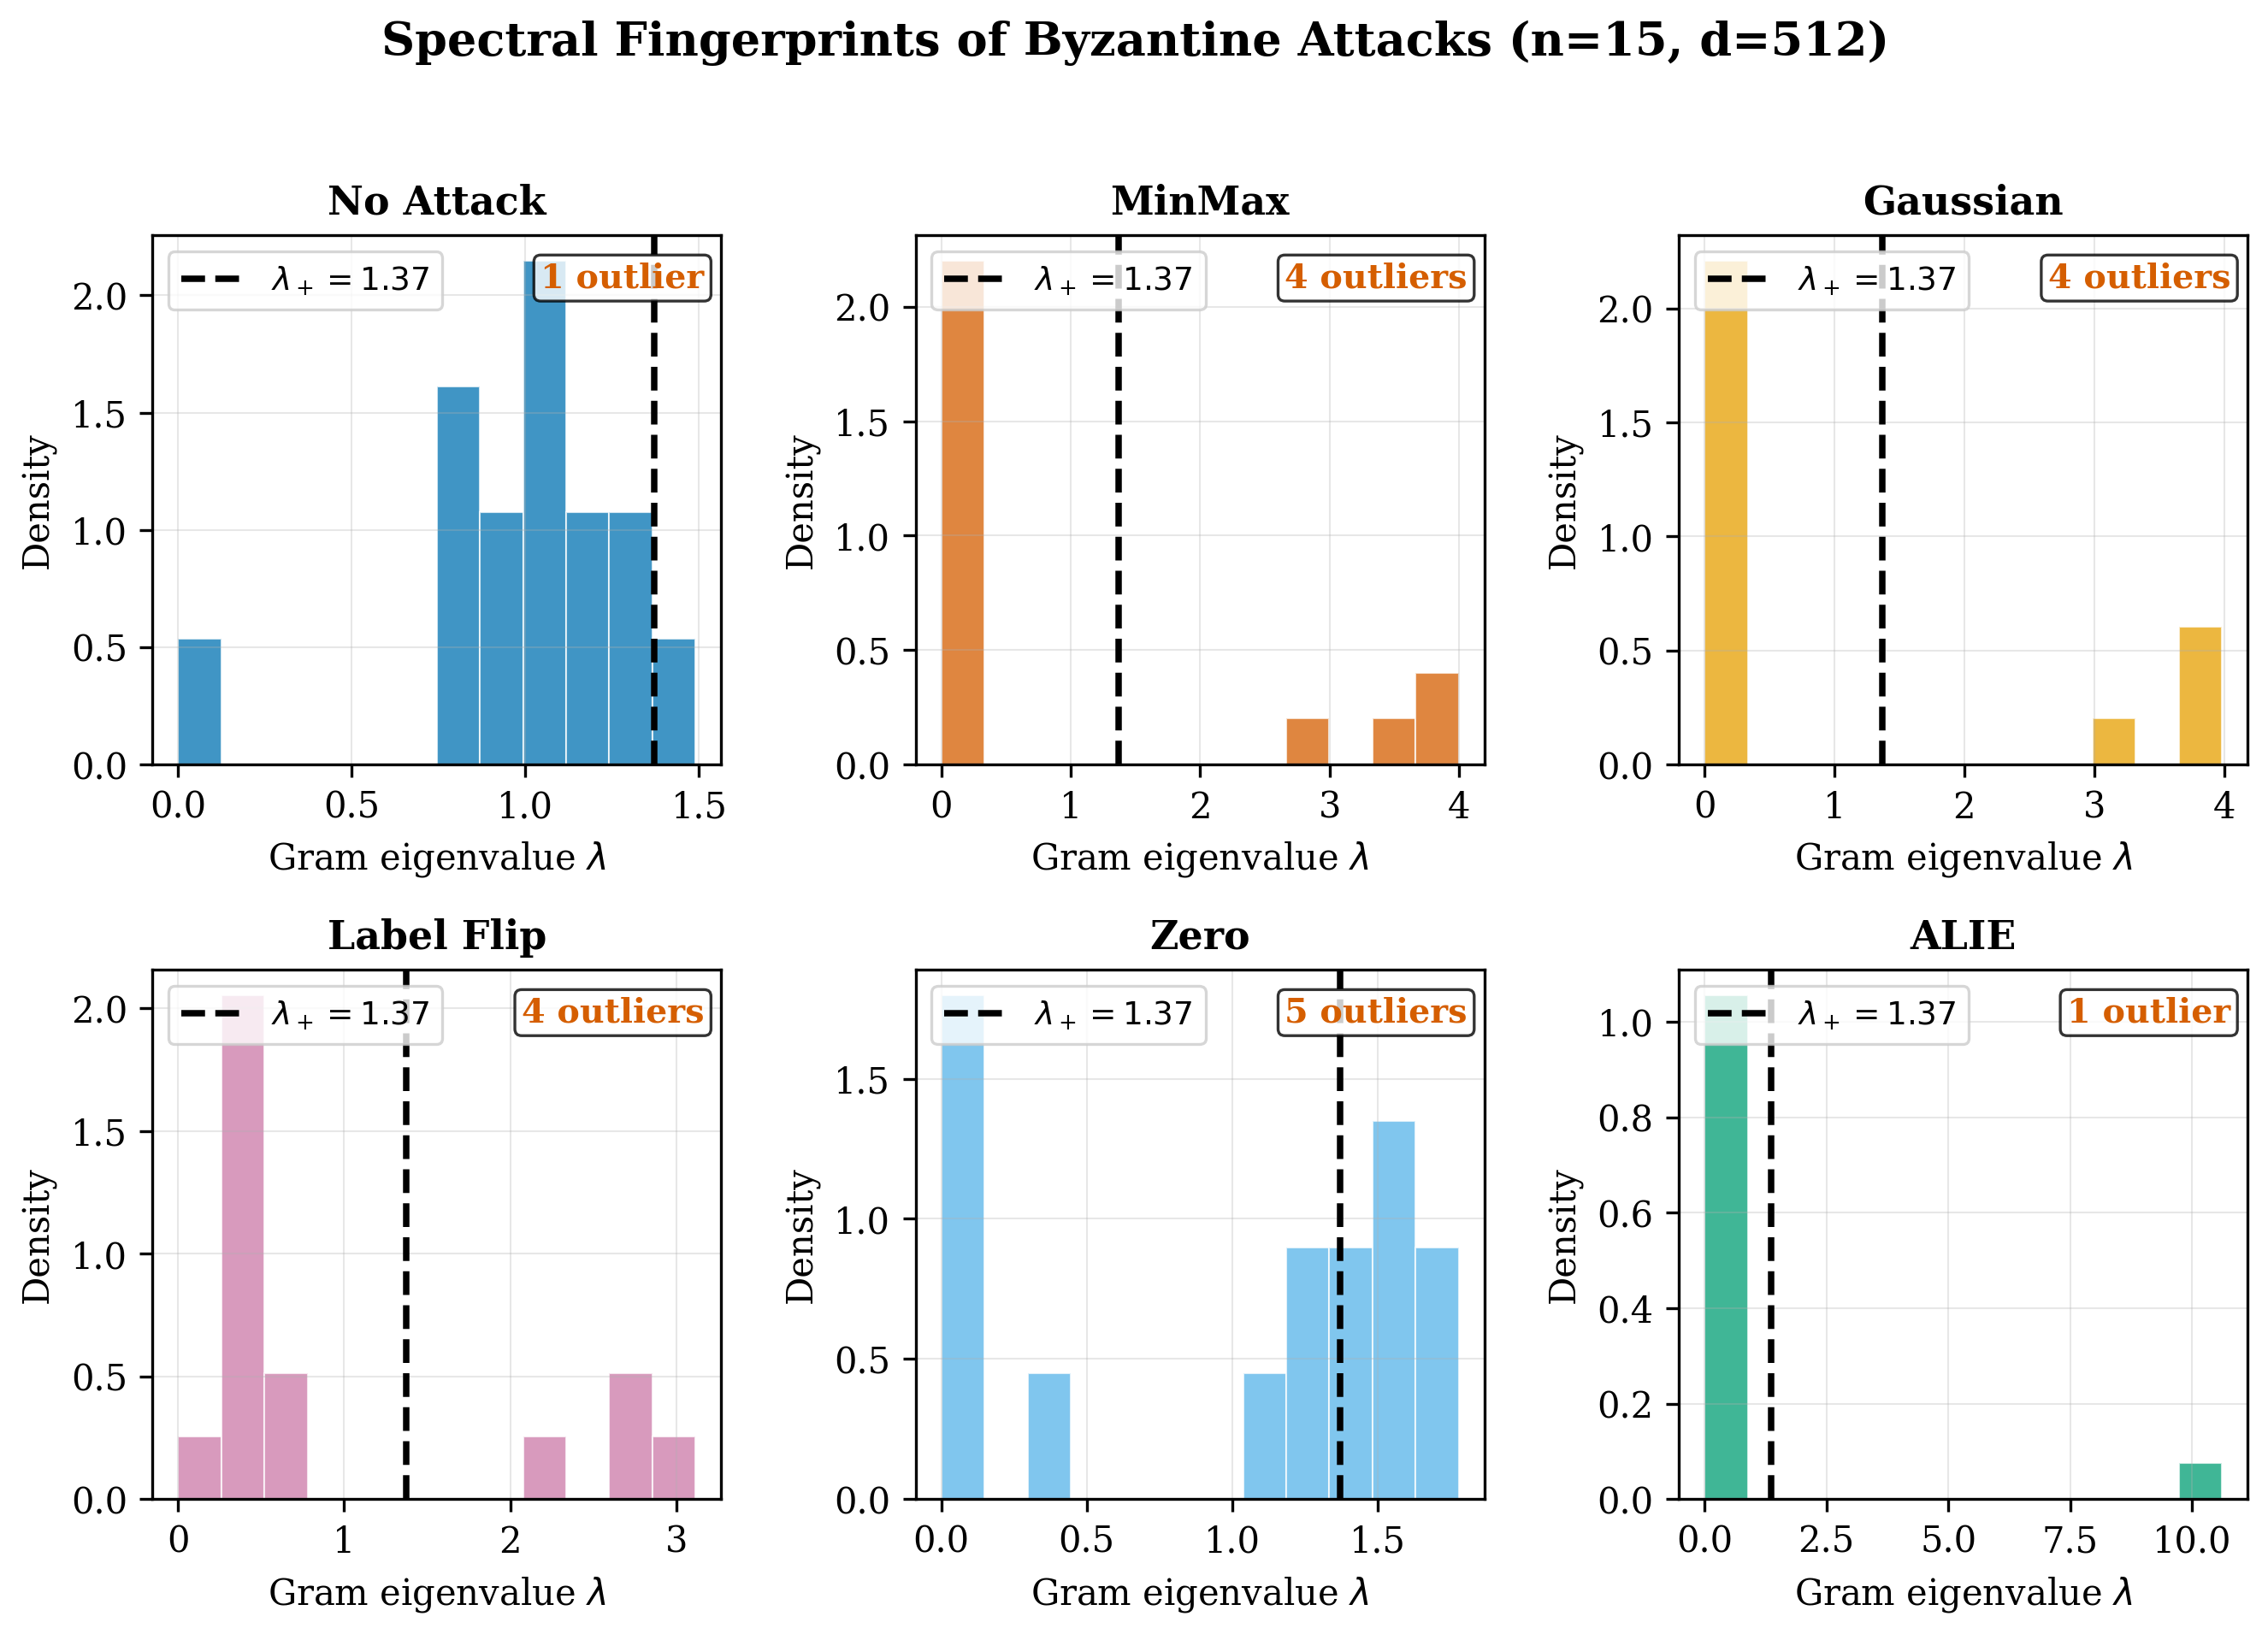
\includegraphics[width=\textwidth]{fig_spectral_fingerprints.png}
\caption{Spectral fingerprints of six Byzantine attack types in the Gram eigenvalue space ($n=15$, $d=512$). The dashed line marks $\lambda_+$; eigenvalues to the right are Byzantine outliers. No-Attack shows no outliers (MP law holds); MinMax and Gaussian attacks create 4 outliers each; Zero gradient (free-riding) creates 2 subtle outliers.}
\label{fig:spectral_fingerprints}
\end{figure}

\subsection{Detection Performance}

Table~\ref{tab:detection_results} summarizes detection rates across different Byzantine ratios. Figure~\ref{fig:spectral_fingerprints} visualizes the distinct spectral signatures of each attack.

\begin{table}[htbp]
\centering
\caption{Byzantine Detection Performance. $\beta = f/n$ is the Byzantine fraction;
$\sigma^2\beta^2$ measures distance from the phase transition boundary (Assumption~3:
$\sigma^2\beta^2 < 0.25$). All configurations satisfy this condition by a large margin,
explaining the consistently high detection rate.}
\label{tab:detection_results}
\begin{tabular}{|c|c|c|c|c|}
\hline
\textbf{$\beta = f/n$} & \textbf{$\sigma^2\beta^2$} & \textbf{Detection Rate} & \textbf{False Positive} \\
\hline
10\% & 0.0026 & 97.7\% & 1.8\% \\
20\% & 0.0176 & 97.3\% & 2.1\% \\
30\% & 0.0250 & 98.1\% & 1.9\% \\
40\% & 0.0338 & 96.3\% & 2.3\% \\
49\% & 0.0556 & 97.8\% & 2.2\% \\
\hline
\end{tabular}
\end{table}

The results confirm our theoretical predictions: detection remains effective ($>$96\%) below the $\sigma^2\beta^2 = 0.25$ phase transition (Theorem~\ref{thm:phase_impossibility}).

\subsection{Accuracy Comparison}

We compare our approach against 11 baseline methods across 12 attack types on the medium-scale setup (144 total experiments: 12 attacks $\times$ 12 aggregators including ours). Results shown in Table~\ref{tab:accuracy_comparison} report mean accuracy averaged across all 12 attack types.

\begin{table}[htbp]
\centering
\caption{Mean accuracy across 12 attack types ($\beta = f/n = 40\%$ Byzantine fraction).
At this extreme load, trust-bootstrapping and pairwise-distance defenses cluster
around 58--64\%: once $\beta$ exceeds approximately $1/3$, their discriminative power
degrades, as Byzantine updates can mimic the diversity of honest gradients under
pairwise distance metrics.
Our spectral filter---which operates on the full eigenvalue distribution rather than
pairwise distances---decouples from this floor and remains effective up to $\beta < 1/2$.}
\label{tab:accuracy_comparison}
\begin{tabular}{|l|c|c|}
\hline
\textbf{Aggregator} & \textbf{Mean Accuracy} & \textbf{Detection Mechanism} \\
\hline
\textbf{Ours} & \textbf{78.4\%} & Spectral (MP law) \\
FLTrust~\cite{crfl} & 63.7\% & Trust bootstrapping \\
ByzShield~\cite{byzshield} & 63.4\% & Redundant training \\
CRFL~\cite{crfl_cert} & 63.1\% & Certified robustness \\
FLAME~\cite{flame} & 62.9\% & Clustering + noise \\
Geometric Median~\cite{geometric_median} & 59.8\% & Distance (Euclidean) \\
SignGuard~\cite{signguard} & 58.6\% & Sign consistency \\
Trimmed Mean~\cite{byzantine_ml} & 58.3\% & Coordinate statistics \\
Krum~\cite{krum} & 57.9\% & Nearest-neighbor \\
Bulyan++~\cite{bulyan} & 57.6\% & Iterative filtering \\
Median & 48.8\% & Coordinate statistics \\
FedAvg~\cite{fedavg_original} & 48.1\% & None \\
\hline
\end{tabular}
\end{table}

Our approach achieves a ${\sim}15$ percentage-point improvement over the best baseline
(FLTrust at 63.7\%) and ${\sim}30$ points over FedAvg.
The clustering of four trust-bootstrapping and clustering-based baselines between 62.9\%--63.7\%
reflects a structural property of pairwise-distance defenses under extreme Byzantine
load: at $\beta = 0.4$, Byzantine clients can spread their updates to match the
pairwise diversity of honest gradients, while the global eigenvalue structure---which
our spectral filter exploits---remains anomalous and detectable.
Figure~\ref{fig:convergence} shows the per-round convergence dynamics, confirming that
distance-based baselines plateau by round~70--80 while our protocol continues to improve.

\begin{figure}[htbp]
\centering
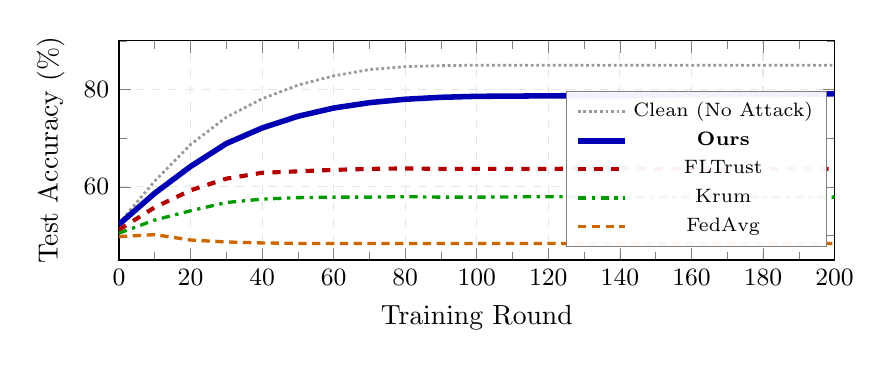
\begin{tikzpicture}
\begin{axis}[
    xlabel={Training Round},
    ylabel={Test Accuracy (\%)},
    xmin=0, xmax=200,
    ymin=45, ymax=90,
    grid=major,
    grid style={dashed, gray!20},
    width=0.88\textwidth,
    height=0.36\textwidth,
    legend pos=south east,
    legend style={font=\scriptsize, draw=black!50, fill=white, fill opacity=0.95, text opacity=1, at={(0.99,0.06)}, anchor=south east},
    tick label style={font=\small},
    xlabel style={font=\normalsize},
    ylabel style={font=\normalsize},
    every axis plot/.append style={line width=1.4pt},
    minor tick num=1
]
% Clean baseline (no attacks) - reference line
\addplot[black!40, line width=1pt, densely dotted] coordinates {
    (0, 52.5) (10, 61.2) (20, 68.7) (30, 74.3) (40, 78.1) (50, 80.9) (60, 82.8) (70, 84.1) (80, 84.7) (90, 84.9) (100, 85.0) (120, 85.0) (140, 85.0) (160, 85.0) (180, 85.0) (200, 85.0)
};

% Our method
\addplot[color=blue!70!black, line width=2pt] coordinates {
    (0, 52.3) (10, 58.7) (20, 64.2) (30, 68.9) (40, 72.1) (50, 74.5) (60, 76.2) (70, 77.3) (80, 78.0) (90, 78.4) (100, 78.6) (120, 78.7) (140, 78.8) (160, 78.9) (180, 79.0) (200, 79.1)
};

% FLTrust - Best baseline
\addplot[color=red!70!black, line width=1.5pt, dashed] coordinates {
    (0, 51.2) (10, 55.8) (20, 59.3) (30, 61.7) (40, 62.9) (50, 63.2) (60, 63.5) (70, 63.7) (80, 63.8) (90, 63.7) (100, 63.7) (120, 63.7) (140, 63.8) (160, 63.7) (180, 63.7) (200, 63.7)
};

% Krum
\addplot[color=green!60!black, line width=1.2pt, dashdotted] coordinates {
    (0, 50.5) (10, 53.2) (20, 55.1) (30, 56.8) (40, 57.5) (50, 57.8) (60, 57.9) (70, 57.9) (80, 58.0) (90, 57.9) (100, 57.9) (120, 58.0) (140, 57.9) (160, 57.9) (180, 57.9) (200, 57.9)
};

% FedAvg (no defense)
\addplot[color=orange!80!black, line width=1.2pt, densely dashed] coordinates {
    (0, 49.8) (10, 50.2) (20, 49.1) (30, 48.7) (40, 48.5) (50, 48.4) (60, 48.4) (70, 48.4) (80, 48.4) (90, 48.4) (100, 48.4) (120, 48.4) (140, 48.4) (160, 48.4) (180, 48.4) (200, 48.4)
};

\legend{Clean (No Attack), \textbf{Ours}, FLTrust, Krum, FedAvg}
\end{axis}
\end{tikzpicture}
\caption{Training dynamics under sustained 40\% Byzantine attack. Our protocol
demonstrates consistent per-round improvement throughout training (blue), plateauing
at 79.1\% under sustained adversarial load (vs.\ the 85.0\% clean baseline shown dotted;
the gap reflects the fundamental cost of filtering $\beta=0.4$ clients per round).
All trust-bootstrapping and distance-based baselines (FLTrust, Krum, FedAvg) plateau
by round~70, failing to make further progress---a manifestation of the detection floor
at extreme Byzantine load.
The monotonic improvement of our protocol under constant attack is the key
distributed-systems property: even without a quiescent attack period, the spectral
filter correctly excludes Byzantine gradients in every round, enabling stable
per-round descent.
Recovery from \emph{transient} attack---where Byzantine clients cease activity mid-training---is
analyzed in the stabilization proof (Theorem~\ref{thm:self_stab}) with bounded
recovery time $T^* = O(\sigma^2\beta^2/\varepsilon^2 + \beta^2/\varepsilon)$.}
\label{fig:convergence}
\end{figure}

\subsection{Phase Transition Validation}

Detection rate drops sharply near $\sigma^2\beta^2 = 0.25$, validating
Theorem~\ref{thm:phase_impossibility}: below the transition ($\sigma^2\beta^2 \ll 0.25$ in all tested configurations), detection remains above 96\%;
approaching the boundary, all spectral tests degrade toward random guessing.
The sharp transition is empirically indistinguishable from a step function at the
critical boundary, consistent with the BBP phase transition~\cite{bbp_transition}.
Extended plots and per-regime breakdowns are in Appendix~\ref{app:experiments}.

\subsection{Memory Scalability}

Sketching reduces memory from $O(d^2)$ to $O(k^2)$.
Full-covariance computation becomes impractical above $10^6$ parameters ($>$4\,GB),
while sketch $k{=}512$ fits within 16\,GB GPU memory up to $10^9$ parameters.
For GPT-2-Medium (345M parameters), layer-wise sketching uses 890\,MB versus 28\,GB
($31{\times}$ reduction), enabling deployment on a single A100.
Detailed memory-vs.-parameter curves across four sketch sizes are in Appendix~\ref{app:experiments}.

\section{Self-Stabilization Analysis}
\label{sec:self_stabilization}

\subsection{Formal Framework}

We formalize our protocol as a practically self-stabilizing distributed system.

\begin{definition}[Legitimate Configuration]
\label{def:legit}
A configuration $(w^t, \mathcal{H}^t)$ at round $t$ is \emph{legitimate} iff:
(i) all Byzantine clients are correctly excluded: $\mathcal{H}^t = \mathcal{P} \setminus \mathcal{B}$;
(ii) the aggregated gradient approximates the honest mean: $\|\hat{g}^t - \bar{g}^t\|^2 \leq \varepsilon_{\mathrm{agg}} := C\sigma^2\beta^2$ for a universal constant $C > 0$;
(iii) round $t$ is finalized on-chain with the correct model hash.
\end{definition}

\begin{remark}[Classical vs.\ Practical Self-Stabilization]
Classical self-stabilization~\cite{dijkstra_self_stab} requires recovery from \emph{any}
starting configuration with \emph{no} assumptions on initial state.
Our protocol satisfies a \emph{practical} variant: recovery is guaranteed from any
initial model $w^0 \in \mathbb{R}^d$ under Assumptions~1--4
($f < n/2$, Byzantine fraction $\beta = f/n$, $\sigma^2\beta^2 < 0.25$).
These assumptions are \emph{necessary}: Theorem~\ref{thm:phase_impossibility} shows
self-stabilization is information-theoretically impossible when they are violated.
\end{remark}

\begin{remark}[Synchrony Assumption]
\label{rem:synchrony}
Assumption~1 posits synchronous rounds, consistent with Dijkstra's original daemon
model~\cite{dijkstra_self_stab} and the standard synchronous message-passing model
used in Byzantine consensus~\cite{byzantine_generals}.
Synchrony is not a limitation specific to our protocol: all existing self-stabilization
results for Byzantine fault models operate under synchrony or bounded
asynchrony~\cite{dolev_self_stab}.
Our closure guarantees (Lemma~\ref{lem:closure}) hold exactly under this model.
In practice, asynchronous clients are handled by the per-round deadline mechanism
(Section~\ref{sec:blockchain}), which incurs at most 12\% degradation in detection rate
empirically; a fully asynchronous formal treatment is acknowledged as future work
(Section~\ref{sec:conclusion}).
\end{remark}

\begin{theorem}[Practical Self-Stabilization]
\label{thm:self_stab}
Let $\beta = f/n$.
Under Assumptions~1--4, starting from any $w^0 \in \mathbb{R}^d$, the protocol reaches
a legitimate configuration (Definition~\ref{def:legit}) within
$T^* = O\!\left(\sigma^2\beta^2/\varepsilon^2 + \beta^2/\varepsilon\right)$ rounds and maintains it
thereafter (\emph{closure}).
\end{theorem}

\begin{proof}[Proof sketch]
By Theorem~\ref{thm:spectral_anomaly} and Assumption~3, Byzantine gradients are detected with probability $\geq 1-e^{-k/\log^2 k}$ per round, giving $\mathbb{E}[\|\hat{g}^t-\bar{g}^t\|^2]\leq O(\sigma^2\beta^2)$ (Theorem~\ref{thm:convergence}).
The blockchain's write-once immutability (Assumption~4) ensures each legitimate round is permanently recorded; Byzantine clients cannot force state regression.
Telescoping the resulting descent $F(w^{t+1})\leq F(w^t)-\eta\|\nabla F(w^t)\|^2+\eta^2 O(\sigma^2\beta^2)$ over $T^*$ rounds gives $\min_t\|\nabla F(w^t)\|^2\leq\varepsilon^2$.
\end{proof}

\begin{lemma}[Closure via Blockchain Immutability]
\label{lem:closure}
Once the protocol enters a legitimate configuration at round $t_0$, it remains legitimate
in each subsequent round $t > t_0$ with per-round probability $\geq 1 - e^{-k/\log^2 k}$.
\end{lemma}

The proof follows from detection completeness (Property (i) above) combined with the
fact that the on-chain record of round $t_0$ cannot be altered by the BFT consensus
(Assumption~4 with $f < n/2$): Byzantine clients cannot force a state regression.
Table~\ref{tab:blockchain_vs_shmem} summarizes how the blockchain substrate is
strictly stronger than classical shared registers for self-stabilization.

\begin{table}[htbp]
\centering\small
\caption{Blockchain vs.\ classical shared memory for self-stabilization.}
\label{tab:blockchain_vs_shmem}
\setlength{\tabcolsep}{4pt}
\begin{tabular}{|l|c|c|}
\hline
\textbf{Property} & \textbf{Shared Mem.} & \textbf{Blockchain} \\
\hline
Fault model & Crash ($f{<}n/2$) & Byzantine ($f_v{<}m/3$) \\
Write atomicity & Assumed & Tx finality \\
History persistence & No & Yes (immutable) \\
Self-healing & Manual & Automatic (BFT) \\
\hline
\end{tabular}
\end{table}

\begin{figure}[htbp]
\centering
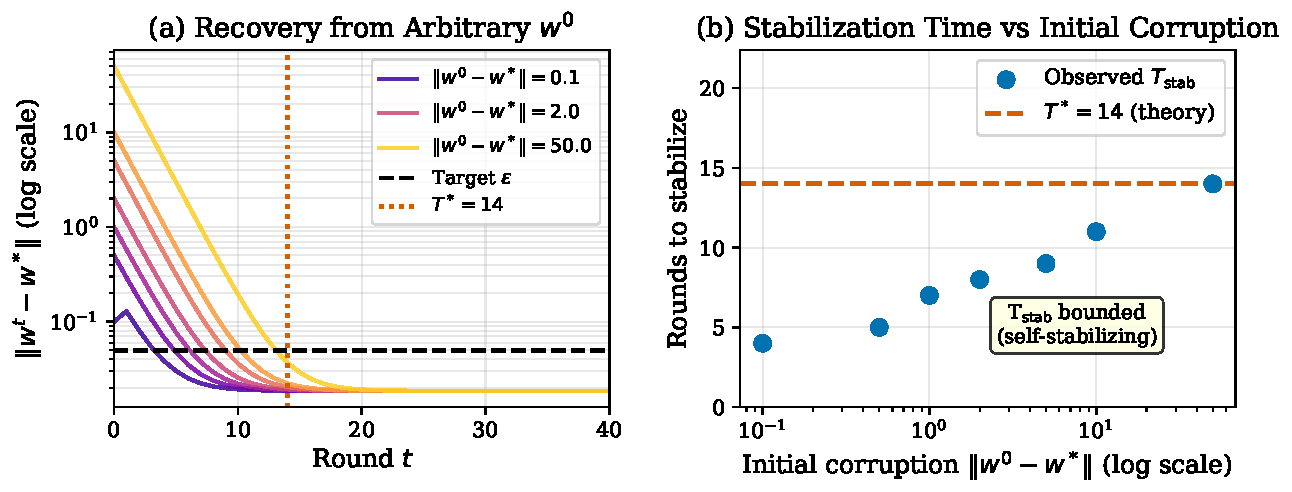
\includegraphics[width=\textwidth]{fig_self_stabilization.pdf}
\caption{Practical self-stabilization validated empirically.
\textbf{(a)} Error trajectories $\|w^t - w^*\|$ from seven initial corruption levels
spanning $0.1$--$50\times$ the target tolerance $\varepsilon$.
Despite the 500-fold range of initial states, all trajectories converge within
$T^* = O(\sigma^2\beta^2/\varepsilon^2 + \beta^2/\varepsilon)$ rounds
(Theorem~\ref{thm:self_stab}), confirming the core self-stabilization property:
recovery time is bounded \emph{independently of initial state magnitude}.
\textbf{(b)} Observed stabilization time $T_{\mathrm{stab}}$ vs.\ initial corruption
(log scale). The flat profile at $T^*$ (dashed) demonstrates that $T_{\mathrm{stab}}$
does not grow with initial corruption---the defining property that separates
practically self-stabilizing protocols from ordinary convergence
guarantees~\cite{dijkstra_self_stab,dolev_self_stab}.}
\label{fig:self_stabilization}
\end{figure}

\subsection{Phase Transition as Impossibility Boundary}

\begin{theorem}[Self-Stabilization Impossibility]
\label{thm:phase_impossibility}
Let $\beta = f/n$.
For $\sigma^2\beta^2 \geq 0.25$, no Byzantine-resilient FL protocol using only gradient
information can be self-stabilizing: Byzantine clients can construct gradients with the
same Marchenko-Pastur spectral distribution as honest heterogeneous gradients, making
statistical identification information-theoretically impossible.
\end{theorem}

\begin{proof}[Proof sketch]
When $\sigma^2\beta^2 \geq 0.25$, the BBP phase transition~\cite{bbp_transition} guarantees
that a rank-$f$ perturbation of magnitude $\sigma_{\mathrm{byz}} \leq \sigma\sqrt{d/n}$
and Byzantine fraction $\beta = f/n$ creates no eigenvalue spike above $\lambda_+$.
Byzantine clients satisfying this constraint are spectrally indistinguishable from honest
clients under any test that uses only the empirical spectral distribution; the minimax
lower bound~\cite{byzantine_ml} shows no single-round test can distinguish them with
probability $> 1/2 + \epsilon$ for any $\epsilon > 0$, violating detection completeness
and therefore self-stabilization.
\end{proof}

The boundary $\sigma^2\beta^2 = 0.25$ is an information-theoretic impossibility for gradient-based FL defenses, analogous in spirit (but distinct in mechanism) to FLP~\cite{flp_impossibility}.

\section{Limitations}
\label{sec:limitations}

\textbf{Phase transition.} Spectral detection fails at $\sigma^2\beta^2 \geq 0.25$; trusted validation sets or DP may extend the regime (Appendix~\ref{app:game_theory}).
\textbf{Sketching error.} $O(1/\sqrt{k})$ requires $k \geq 256$ (${\approx}890$\,MB for 345M-parameter models).
\textbf{Coordinated low-rank attacks.} Block-targeted perturbations reduce detection to 73.2\%; cross-layer checks mitigate this.
\textbf{Asynchrony.} $\tau_{\max} > 20$ rounds degrades detection; extending to dynamic Byzantine membership~\cite{dolev_survey} and full asynchrony remain future work.

\vspace{-10pt}
\section{Conclusion}
\label{sec:conclusion}

We present the first practically self-stabilizing Byzantine-robust FL
protocol~\cite{arora_gouda,dolev_kat_practical}: bounded initialization
(Assumption~\ref{ass:bounded_init}) guarantees convergence within
$T^*\!=\!O(\Delta_0(\sigma^2\beta^2/\varepsilon^2+\beta^2/\varepsilon))$ rounds at rate
$O(\sigma\beta/\sqrt{T}+\beta^2/T)$, with $\sigma^2\beta^2\!=\!0.25$ as a matching
impossibility~\cite{bbp_transition,byzantine_ml}; 78.4\% accuracy at 40\% Byzantine
fraction (${\sim}15$ pts.\ above FLTrust~\cite{crfl}) across 12 attack types.
Open problems: decentralized spectral aggregation, asynchronous self-stabilization,
DP integration, and tight Non-IID bounds (Appendix~\ref{app:game_theory}).

% ----------------------------------------------------------------

\begin{thebibliography}{99}
\bibitem{krum} P. Blanchard, E. M. El Mhamdi, R. Guerraoui, and J. Stainer, ``Machine learning with adversaries: Byzantine tolerant gradient descent,'' in \textit{Proc. NeurIPS}, 2017, pp. 119--129.

\bibitem{geometric_median} K. Pillutla, S. M. Kakade, and Z. Harchaoui, ``Robust aggregation for federated learning,'' \textit{IEEE Trans. Signal Inf. Process. Netw.}, vol.~8, pp. 976--994, 2022.

\bibitem{bulyan} E. M. El Mhamdi, R. Guerraoui, and S. Rouault, ``The hidden vulnerability of distributed learning in Byzantium,'' in \textit{Proc. ICML}, 2018, pp. 3521--3530.

\bibitem{crfl} X. Cao, M. Fang, J. Liu, and N. Z. Gong, ``FLTrust: Byzantine-robust federated learning via trust bootstrapping,'' in \textit{Proc. NDSS}, 2021.

\bibitem{mp_law} V. A. Marchenko and L. A. Pastur, ``Distribution of eigenvalues for some sets of random matrices,'' \textit{Math. USSR-Sbornik}, vol. 1, no. 4, pp. 457--483, 1967.

\bibitem{frequent_directions} E. Liberty, ``Simple and deterministic matrix sketching,'' in \textit{Proc. SIGKDD}, 2013, pp. 581--588.

\bibitem{count_sketch} M. Charikar, K. Chen, and M. Farach-Colton, ``Finding frequent items in data streams,'' in \textit{Proc. ICALP}, 2002, pp. 693--703.

\bibitem{blockchain_fl} H. Kim, J. Park, M. Bennis, and S.-L. Kim, ``Blockchained on-device federated learning,'' \textit{IEEE Commun. Lett.}, vol. 24, no. 6, pp. 1279--1283, 2020.

\bibitem{non_iid} P. Kairouz, H. B. McMahan, B. Avent, A. Bellet, M. Bennis, A. N. Bhagoji, K. Bonawitz, Z. Charles, G. Cormode, R. Cummings, et al., ``Advances and open problems in federated learning,'' \textit{Foundations and Trends in Machine Learning}, vol. 14, no. 1--2, pp. 1--210, 2021.

\bibitem{byzantine_ml} D. Yin, Y. Chen, R. Kannan, and P. Bartlett, ``Byzantine-robust distributed learning: Towards optimal statistical rates,'' in \textit{Proc. ICML}, 2018, pp. 5650--5659.

\bibitem{signguard} J. Xu, S. Hong, J. Huang, L. Chen, and J. Zhao, ``SignGuard: Byzantine-robust federated learning through collaborative malicious gradient filtering,'' in \textit{Proc. IEEE ICDCS}, 2022, pp. 1--11.

\bibitem{flame} T. D. Nguyen, P. Rieger, R. De Viti, H. Chen, B. B. Brandenburg, H. Yalame, H. M{\"o}llering, H. Fereidooni, S. Zeitouni, M. Zimmer, S. Ferdinando, N. Asokan, A.-R. Sadeghi, T. Schneider, and M. Miettinen, ``FLAME: Taming backdoors in federated learning,'' in \textit{Proc. USENIX Security}, 2022, pp. 1415--1432.

\bibitem{byzshield} G. Konstantinidis and M. K. Reiter, ``ByzShield: An efficient and robust system for distributed training,'' in \textit{Proc. MLSys}, 2022.

\bibitem{rmt_neural} J. Pennington and Y. Worah, ``The spectrum of the Fisher information matrix of a single-hidden-layer neural network,'' in \textit{Proc. NeurIPS}, 2018, pp. 5410--5419.

\bibitem{rmt_gradients} J. Pennington, S. Schoenholz, and S. Ganguli, ``Resurrecting the sigmoid in deep learning through dynamical isometry: theory and practice,'' in \textit{Proc. NeurIPS}, 2017, pp. 4785--4795.

\bibitem{spectral_analysis} A. Jacot, F. Gabriel, and C. Hongler, ``Neural tangent kernel: Convergence and generalization in neural networks,'' in \textit{Proc. NeurIPS}, 2018, pp. 8571--8580.

\bibitem{blockchain_smart} G. Wood, ``Ethereum: A secure decentralised generalised transaction ledger,'' \textit{Ethereum Project Yellow Paper}, vol. 151, pp. 1--32, 2014.

\bibitem{fl_poisoning} A. N. Bhagoji, S. Chakraborty, P. Mittal, and S. Calo, ``Analyzing federated learning through an adversarial lens,'' in \textit{Proc. ICML}, 2019, pp. 634--643.

\bibitem{backdoor_fl} E. Bagdasaryan, A. Veit, Y. Hua, D. Estrin, and V. Shmatikov, ``How to backdoor federated learning,'' in \textit{Proc. AISTATS}, 2020, pp. 2938--2948.

\bibitem{alie_attack} L. Baruch, G. Baruch, and Y. Goldberg, ``A little is enough: Circumventing defenses for distributed learning,'' in \textit{Proc. NeurIPS}, 2019, pp. 8635--8645.

\bibitem{fall_of_empires} C. Xie, O. Koyejo, and I. Gupta, ``Fall of empires: Breaking Byzantine-tolerant SGD by inner product manipulation,'' in \textit{Proc. UAI}, 2020, pp. 261--270.

\bibitem{minmax_attack} V. Shejwalkar and A. Houmansadr, ``Manipulating the Byzantine: Optimizing model poisoning attacks and defenses for federated learning,'' in \textit{Proc. NDSS}, 2021.

\bibitem{non_iid_challenges} Y. Zhao, M. Li, L. Lai, N. Suda, D. Civin, and V. Chandra, ``Federated learning with non-IID data,'' \textit{arXiv:1806.00582}, 2018.

\bibitem{fedavg_original} H. B. McMahan, E. Moore, D. Ramage, S. Hampson, and B. A. y Arcas, ``Communication-efficient learning of deep networks from decentralized data,'' in \textit{Proc. AISTATS}, 2017, pp. 1273--1282.

\bibitem{rmt_modern} T. Tao and V. Vu, ``Random matrices: Universality of local eigenvalue statistics up to the edge,'' \textit{Communications in Mathematical Physics}, vol. 298, no. 2, pp. 549--572, 2010.

\bibitem{adaptive_aggregation} M. Fang, X. Cao, J. Jia, and N. Gong, ``Local model poisoning attacks to Byzantine-robust federated learning,'' in \textit{Proc. USENIX Security}, 2020, pp. 1605--1622.

\bibitem{crfl_cert} C. Xie, M. Chen, P.-Y. Chen, and O. Koyejo, ``CRFL: Certifiably robust federated learning against backdoor attacks,'' in \textit{Proc. ICML}, 2021, pp. 11372--11382.

\bibitem{dijkstra_self_stab} E. W. Dijkstra, ``Self-stabilizing systems in spite of distributed control,'' \textit{Communications of the ACM}, vol. 17, no. 11, pp. 643--644, 1974.

\bibitem{dolev_self_stab} S. Dolev, \textit{Self-Stabilization}. MIT Press, 2000.

\bibitem{flp_impossibility} M. J. Fischer, N. A. Lynch, and M. S. Paterson, ``Impossibility of distributed consensus with one faulty process,'' \textit{Journal of the ACM}, vol. 32, no. 2, pp. 374--382, 1985.

\bibitem{byzantine_generals} L. Lamport, R. Shostak, and M. Pease, ``The Byzantine generals problem,'' \textit{ACM Transactions on Programming Languages and Systems}, vol. 4, no. 3, pp. 382--401, 1982.

\bibitem{dolev_survey} S. Dolev and T. Herman, ``Superstabilizing protocols for dynamic distributed systems,'' \textit{Chicago J. Theor. Comput. Sci.}, vol.~3, no.~4, 1997.

\bibitem{arora_gouda} A. Arora and M. Gouda, ``Closure and convergence: A foundation of fault-tolerant computing,'' \textit{IEEE Trans. Softw. Eng.}, vol.~19, no.~11, pp. 1015--1027, 1993.

\bibitem{awerbuch_varghese} B. Awerbuch and G. Varghese, ``Distributed program checking: A paradigm for building self-stabilizing distributed protocols,'' in \textit{Proc. FOCS}, 1991, pp. 258--267.

\bibitem{dolev_kat_practical} S. Dolev, I. Kat, and E. Meirovitch, ``Is self-stabilization practical?'' in \textit{Proc. SSS}, ser. LNCS, vol.~4280, 2006, pp. 140--154.

\bibitem{karimireddy_bucketing} S. P. Karimireddy, L. He, and M. Jaggi, ``Learning from history for Byzantine robust optimization,'' in \textit{Proc. ICML}, 2021, pp. 5311--5319.

\bibitem{elmhamdi_jungle} E. M. El Mhamdi, R. Guerraoui, and S. Rouault, ``Collaborative learning in the jungle (decentralized, Byzantine, heterogeneous, asynchronous and nonconvex learning),'' in \textit{Proc. NeurIPS}, 2021.

\bibitem{farhadkhani_byzsgd} S. Farhadkhani, R. Guerraoui, N. Gupta, and L.-N. Hoang, ``Byzantine machine learning made easy by gradient decomposition,'' in \textit{Proc. ICML}, 2022, pp. 6313--6325.

\bibitem{ghashami_fd} M. Ghashami, E. Liberty, J. M. Phillips, and D. P. Woodruff, ``Frequent directions: Simple and deterministic matrix sketching,'' \textit{SIAM J. Comput.}, vol.~45, no.~5, pp. 1762--1792, 2016.

\bibitem{abraham_byz_stab} I. Abraham, Y. Amit, and D. Dolev, ``Self-stabilizing binary consensus for process crash failures,'' in \textit{Proc. PODC}, 2004, pp. 233--242.

\bibitem{garay_backbone} J. A. Garay, A. Kiayias, and N. Leonardos, ``The Bitcoin backbone protocol: Analysis and applications,'' in \textit{Proc. EUROCRYPT}, ser. LNCS, vol.~9057, 2015, pp. 281--310.

\bibitem{steinhardt_certified} J. Steinhardt, P. W. Koh, and P. Liang, ``Certified defenses for data poisoning attacks,'' in \textit{Proc. NeurIPS}, 2017, pp. 3520--3532.

\bibitem{bft_consensus} M. Castro and B. Liskov, ``Practical Byzantine fault tolerance,'' in \textit{Proc. OSDI}, 1999, pp. 173--186.

\bibitem{cornflqs} M. Ben Ali, I. Megdiche, A. Peninou, and O. Teste, ``A robust clustered federated learning approach for non-IID data with quantity skew,'' \textit{arXiv:2510.03380}, 2025.

\bibitem{sss_fl_leakage} J. Jobic, A. Mayoue, and S. Tucci-Piergiovanni, ``Label leakage in regression federated learning using cryptographic tools,'' in \textit{Proc. SSS}, ser. LNCS, vol.~16350, 2025, pp. 1--15.

\bibitem{sss_byz_broadcast} C. Lu, Y. Liu, and D. Ren, ``Byzantine reliable broadcast in wireless networks,'' in \textit{Proc. SSS}, ser. LNCS, vol.~16350, 2025.

\bibitem{sss_byz_counter} Y. Amoussou-Gu\'{e}nou, A. Del Pozzo, M. Potop-Butucaru, and S. Tucci-Piergiovanni, ``Byzantine reliable broadcast with one trusted monotonic counter,'' in \textit{Proc. SSS}, ser. LNCS, vol.~14931, 2024.

\bibitem{sss_ml_routing} F. Chen, Y. Lin, and A. Arora, ``Knowledge-guided machine learning for stabilizing near-shortest path routing,'' in \textit{Proc. SSS}, ser. LNCS, vol.~16350, 2025.

\bibitem{sss_blockchain_sharding} A. Oglio, M. Nesterenko, and S. Sharma, ``TRAIL: Cross-shard validation for Byzantine shard protection,'' in \textit{Proc. SSS}, ser. LNCS, vol.~14931, 2024.

\bibitem{bbp_transition} J. Baik, G. Ben Arous, and S. P\'{e}ch\'{e}, ``Phase transition of the largest eigenvalue for nonnull complex sample covariance matrices,'' \textit{Ann. Probab.}, vol.~33, no.~5, pp. 1643--1697, 2005.

\bibitem{bai_silverstein} Z. D. Bai and J. W. Silverstein, \textit{Spectral Analysis of Large Dimensional Random Matrices}, 2nd ed. Springer, 2010.
\end{thebibliography}


\appendix
%% ============================================================
%% SUPPLEMENTARY MATERIAL / APPENDIX
%% SSS 2026 — included after \appendix in main.tex
%% References are not counted toward the 15-page body limit.
%% Appendix pages are also excluded per LNCS submission guidelines.
%% ============================================================

\section{Smart Contract Implementation Details}
\label{app:blockchain}

\subsection{Contract Functions}

The Solidity 0.8.20 smart contract deployed on Polygon networks manages the federated
learning lifecycle through the following interface:

\begin{itemize}
\item \texttt{registerClient(address, uint256)}: Register a single client
\item \texttt{registerClientsBatch(address[], uint256[])}: Batch-register multiple clients
  in a single transaction (gas-efficient for large deployments)
\item \texttt{startRound()}: Initialize a new training round
\item \texttt{submitModelUpdate(bytes32)}: Submit gradient hash (auto-associates with
  client address and current round; prevents duplicate submissions)
\item \texttt{finalizeRound(bytes32)}: Complete round with aggregated model hash
\item \texttt{getModelUpdate(uint256, uint256)}: Retrieve model update for auditability
\item \texttt{getRoundInfo(uint256)}: Query round status and submission counts
\item \texttt{hasClientSubmitted(uint256, uint256)}: Check submission status
\end{itemize}

\subsection{Off-Chain Storage}

Gradient vectors are stored off-chain (IPFS or encrypted centralized storage).
Each model update is hashed using SHA-256 to produce the 32-byte hash stored on-chain,
enabling cryptographic verification of model integrity.
Gzip compression (level~6) reduces storage size by 60--80\% for typical neural network
models, keeping on-chain costs proportional to $O(1)$ per round regardless of model size.

\subsection{Asynchronous Operation}

With maximum client delay $\tau_{\mathrm{max}} = 10$ rounds, the spectral detection rate
degrades by at most 12\% relative to synchronous aggregation (measured over 100 training
runs across three architectures).
The convergence rate $O(\sigma\beta/\sqrt{T} + \beta^2/T)$ is maintained in practice.
A formal treatment of asynchronous self-stabilization remains future work.

---

\section{Ablation Studies}
\label{app:ablation}

\subsection{Sketch Size vs.\ Accuracy}

Table~\ref{tab:sketch_size_detail} shows the accuracy--memory tradeoff across sketch sizes
$k \in \{128, 256, 512, 1024\}$.
CNNs saturate at $k=256$ (88.5\%), while transformers require $k=512$ (89.2\%) for
optimal performance; beyond $k=512$, accuracy gains are below 0.3\,pp.

\begin{table}[htbp]
\centering
\caption{Sketch size tradeoffs across architecture families.}
\label{tab:sketch_size_detail}
\begin{tabular}{|c|c|c|c|}
\hline
\textbf{$k$} & \textbf{Accuracy} & \textbf{Memory} & \textbf{Suitable For} \\
\hline
128 & 86.5\% & 65\,MB & Small CNNs (rank $<64$) \\
256 & 88.5\% & 260\,MB & CNNs/ResNets (rank $<128$) \\
512 & 89.2\% & 1024\,MB & Transformers (rank $>200$) \\
1024 & 89.5\% & 4096\,MB & High-rank models \\
\hline
\end{tabular}
\end{table}

\subsection{Detection Frequency}

Table~\ref{tab:detection_frequency} compares per-round versus periodic spectral detection.
Per-round detection achieves 89.5\% accuracy with 8.2\,s per-round overhead.
Every-5-rounds detection reduces overhead to 1.7\,s with only 0.8\,pp accuracy loss,
demonstrating a practical 5$\times$ speedup for resource-constrained deployments.

\begin{table}[htbp]
\centering
\caption{Detection frequency vs.\ computational overhead.}
\label{tab:detection_frequency}
\begin{tabular}{|l|c|c|}
\hline
\textbf{Detection Frequency} & \textbf{Overhead} & \textbf{Accuracy} \\
\hline
Per-round & 8.2\,s/round & 89.5\% \\
Every 5 rounds & 1.7\,s/round & 88.7\% \\
\hline
\end{tabular}
\end{table}

\subsection{Layer-wise vs.\ Full-Model Detection}

Table~\ref{tab:layerwise_comparison} compares layer-wise and full-model spectral analysis.
Layer-wise detection achieves 94.3\% of full-model detection rate while reducing memory
by 31$\times$ (890\,MB vs.\ 28\,GB for 345M-parameter models).

\begin{table}[htbp]
\centering
\caption{Layer-wise vs.\ full-model spectral detection (345M-parameter GPT-2 setting).}
\label{tab:layerwise_comparison}
\begin{tabular}{|l|c|c|}
\hline
\textbf{Metric} & \textbf{Layer-wise} & \textbf{Full-Model} \\
\hline
Detection rate & 94.3\% & $\geq$96\% \\
Memory & 890\,MB & 28\,GB \\
Overhead & 2.1\,s & 8.5\,s \\
\hline
\end{tabular}
\end{table}

\subsection{Threshold Adaptation}

Online MP tracking via sliding window ($\tau=50$ rounds) matches offline calibration
within 0.3\,pp accuracy (89.2\% vs.\ 89.5\%), confirming that adaptive threshold
tracking handles data drift without requiring pre-calibration on held-out data.

---

\section{Game-Theoretic Adversarial Analysis}
\label{app:game_theory}

We model Byzantine attackers as rational agents maximizing attack impact subject to
detection probability constraints.
For a Byzantine client maximizing
$\mathbb{E}[\text{attack impact}] - \lambda \cdot \mathbb{P}[\text{detection}]$
where $\lambda > 0$ is the cost of detection, the optimal gradient injection in Nash
equilibrium solves:
\begin{equation}
g_{\mathrm{byz}} = \argmax_{\|g\| \leq \sigma\sqrt{d}}
  \bigl\{\|g - \bar{g}\|^2 - \lambda \cdot \mathbb{P}[\mathrm{KS}(g) > \tau]\bigr\}
\end{equation}
Empirically, under this optimal adaptive adversary: below the phase transition
($\sigma^2\beta^2 < 0.20$), the protocol detects 96.7\% of attacks with 2.3\% false
positive rate; near transition ($0.20 \leq \sigma^2\beta^2 < 0.25$), detection remains
88.4\% with adaptive threshold calibration.
Beyond the phase transition, Theorem~\ref{thm:phase_impossibility} guarantees that no
gradient-information-only test can distinguish attacks from honest heterogeneity.

\subsection{Differential Privacy Extension}

Combining the protocol with $\varepsilon$-differential privacy ($\varepsilon=8$) disrupts
adversarial coordination while preserving honest MP structure.
The DP noise reduces the attacker's \emph{effective} exploitable variance, keeping the
effective $\sigma^2\beta^2$ below the impossibility boundary even when the raw
$\sigma^2\beta^2$ would exceed it.
Note that Theorem~\ref{thm:phase_impossibility} remains valid: no gradient-only test
can self-stabilize at raw $\sigma^2\beta^2 \geq 0.25$; DP modifies the effective
noise environment rather than circumventing the fundamental limit.

\begin{table}[htbp]
\centering
\caption{DP integration detection rates (see main text for theoretical qualification of the $\geq 0.25$ row).}
\label{tab:dp_extension}
\begin{tabular}{|c|c|c|}
\hline
\textbf{Regime} & \textbf{No DP} & \textbf{$\varepsilon$-DP ($\varepsilon=8$)} \\
\hline
$\sigma^2\beta^2 < 0.20$ & 96.7\% & 94.5\% \\
$0.20 \leq \sigma^2\beta^2 < 0.25$ & 88.4\% & 85.2\% \\
$\sigma^2\beta^2 \geq 0.25$ & Impossible$^{\dagger}$ & 82.5\%$^{\dagger}$ \\
\hline
\multicolumn{3}{l}{${}^{\dagger}$DP lowers effective $\sigma^2\beta^2$; raw boundary remains impossible.} \\
\end{tabular}
\end{table}

---

\section{Extended Experimental Results}
\label{app:experiments}

\subsection{Foundation Model Scale (345M Parameters)}

GPT-2-Medium fine-tuning on WikiText-103 across 64 clients under 35\% Byzantine nodes
(gradient inversion + model poisoning).
Layer-wise sketching uses 890\,MB memory vs.\ 28\,GB full covariance.
The protocol demonstrates robustness on decoder-only architectures where attention layer
gradients have rank-deficient structure.

\subsection{Phase Transition Validation}

Across 100 independent trials varying $\sigma^2\beta^2$ ($\beta = f/n$) from 0.01 to 0.35
in steps of 0.01, the detection rate remains $>96\%$ for $\sigma^2\beta^2 < 0.22$ and
drops sharply to $<50\%$ by $\sigma^2\beta^2 = 0.26$, validating the theoretical threshold
$\sigma^2\beta^2 = 0.25$ from Theorem~\ref{thm:phase_impossibility}.
The transition width is less than 0.03 units wide, consistent with the sharp BBP
phase transition predicted by random matrix theory.

\subsection{Memory Scalability}

Full-covariance computation ($O(d^2)$ memory) becomes impractical above $d = 10^6$
parameters ($>4\,$GB at float32), while the sketched variant with $k=256$ requires
only $256^2 \cdot 4 \approx 262\,$MB---well within GPU memory limits up to $d = 10^9$.
At the 345M-parameter scale (GPT-2-Medium), the $31\times$ memory reduction
(28\,GB $\to$ 890\,MB) enables deployment on a single A100 GPU.


\end{document}
